%---------------------------------------------------------------------------------------------------
% Theory
%---------------------------------------------------------------------------------------------------
\newpage
\chapter{Theory} 
\section{Basics of Electric Guitars}
\subsubsection{Guitar Components}

\begin{figure}[H]
	\centering 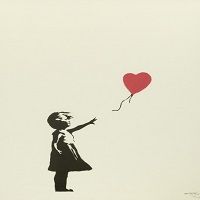
\includegraphics[width=0.8\textwidth]{banksy.jpg}
	\caption[ElectricGuitar]{Components of an electric guitar\footnotemark}
	\label{fig:ElectricGuitar}
\end{figure}
\footnotetext{URL: https://www.guitarchalk.com/wp-content/uploads/2017/07/electric-guitar-parts.jpg [cited 22 August 2018]}

A regular electric guitar consists of six strings and two or three pickups (\ref{fig:ElectricGuitar}).
Acoustic guitars have a hollow soundboard in which the vibration of the strings resonates. As a consequence, the sound is transmitted to the air. Regular electric guitars have a solid-body and depend on electromagnetic
pickups which are turning mechanical vibrations into an electric signal for further amplification.\\
Before the output signal is provided for the processing by external devices, it can be modified
by the volume and tone controls. The volume controller is a potentiometer that regulates the output voltage.
Tone controls consists of a potentiometer connected in series with a capacitor simply acting as a filter.
%In regard to the main goal of this work, there is no further explanation of the controls necessary.
% Not neary describes cause not part of this thesis


\begin{figure}[H]
	\centering 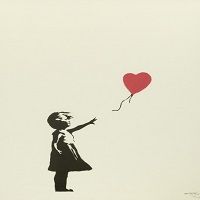
\includegraphics[width=0.5\textwidth]{banksy.jpg}
	\caption[SingleCoil]{Scheme of a single-coil pickup \cite[p 29]{Zollner:2009}}
	\label{fig:SingleCoil}
\end{figure}

For this thesis only passive single coil pickups, as fitted to the majority of electric guitars, are described.
A pickup basically consists of six bar magnets wrapped with a copper-wired coil, see figure (\ref{fig:SingleCoil}).
The magnets produce a stable magnetic field which is disturbed when a string is plucked.
A vibrating string, made of ferromagnetic material, induces an electric Voltage into the coil.\\
According to Faraday's law of induction (see eq. \ref{eq:faraday}) the Voltage $u$ in a wound coil of wire with $n$ turns is proportional to the change of the magnetic flux $\Phi$ over time.


\begin{equation}
u=n \frac{d\Phi}{dt}
\label{eq:faraday}
\end{equation}

\subsubsection{Frequency Range}\label{subsec:FrequencyRange}

The sound from a guitar can be described as a note. Furthermore, every note corresponds to a fundamental frequency.
The fundamental frequencies can be calculated (see eq. \ref{eq:fretFrequencies}).\\
The hearable fundamental frequency $f_{\mathrm{string/fret}}$ depends on the fret played and the frequency $f_{0,\mathrm{string}}$ of the open string that is stroked.
A regular six-string guitar with 24 frets in the standard-tuning (\ref{tab:tableFrequencies}) can generate fundamental frequencies between 82,41\,Hz and 1318,5\,Hz.\\
Besides the fundamental frequencies, an electric guitar produces harmonics at the same time.
Harmonics are integer multiples of the fundamental frequency \cite[p.\,150]{Gorne:2015}. These are overlapped with the fundamental 
frequency in the time domain which leads to the measurable signal form at the output.\\
The total frequency range of an electric guitar is extended by the harmonics up to several kilohertz.
As a limiting factor the total hearable frequency range of a human ear, 16\,Hz to 20\,kHz\,\cite[p.\,28]{Gorne:2015} should be taken into consideration.



\begin{equation}
f_{\mathrm{string/fret}} = f_{0,\mathrm{string}}\cdot \sqrt[12]{2}^{\,\mathrm{fret}}
\label{eq:fretFrequencies}
\end{equation}

\begin{table}[H]
\begin{center}
	\begin{tabular}{|c||c|c|c|c|c|c|}
	\hline 
	\textbf{Open string} & 1(Low) & 2 & 3 & 4 & 5 & 6(High) \\ 
	\hline 
	\textbf{Note} & E & A & D & G & B & E \\ 
	\hline 
	$f_{0,\mathrm{string}}/\mathrm{Hz}$ & 82,41 & 110 & 146,83 & 196,00 & 246,94 & 329,63 \\ 
	\hline 
	\end{tabular} 
\caption[Bla]{Standard tuning of a guitar\footnotemark}
\end{center}
\label{tab:tableFrequencies}
\end{table}
\footnotetext{URL: https://en.wikipedia.org/wiki/Guitar\_tunings [cited 22 August 2018]}




\section{Basics of Audio Engineering}\label{cap:BasicsOfAudio}
\subsubsection{Acoustical Level}

The human ear is not designed for absolute loudness values. The principle of
subjective loudness is based on stimuli-doubling and halving \cite[p.\,3]{Gorne:2015}. Therefore the acoustic
levels are described in logarithmic scale to represent human sensory perception.
It is common to refer to a power of a signal or the intensity of the sound as a "level".
To quantify the sound intensity the most common dimension used is the sound pressure level\,(SPL) $L_{\mathrm{p 0}}$ measured
in decibel.
$L_{\mathrm{p}}$ is defined relative to the smallest sound pressure noticeable of $p_0 = 20 \mu \mathrm{Pa}$ as a reference level (see eq.\,\ref{eq:SPL}).
Table \ref{tab:SPLs} shows a few exemplary sound sources and the resulting SPL at one meter distance.


\begin{equation}
L_{\mathrm{p}} = 20 \mathrm{log} \frac{p}{p_0}\, \mathrm{dB}
\label{eq:SPL}
\end{equation}

\begin{table}[H]
\begin{center}
\begin{tabular}{|c|c||c|c|}
\hline 
\textbf{Sound source} & \textbf{$L_{\mathrm{p}}/\mathrm{dB}$ at 1m} & \textbf{Sound source} & \textbf{$L_{\mathrm{p}}/\mathrm{dB}$ at 1m}  \\ 
\hline 
\hline
Threshold of hearing & 0 & Street traffic & 80 \\ 
\hline 
Quiet rural location at night & 20 & Pneumatic hammer & 100 \\ 
\hline 
Library & 40 & Threshold of pain & 120 \\ 
\hline 
Talking & 60 & Rifle & 140 \\ 
\hline 
\end{tabular} 
\caption[oi]{Example of SPL levels\footnotemark}
\end{center}
\label{tab:SPLs}
\end{table}
\footnotetext{URL: https://www.bsria.co.uk/news/article/acoustic-testing-what-is-actually-measured/ [cited 23 August 2018]}
% calc of Pegel

In audio engineering, the sound levels are defined by electrical levels.
To have a corresponding translation from the acoustic level to the electrical level
volume controls are often designed in a logarithmic scale \cite[p.\,34]{Gorne:2015}.
In addition to that, the electrical levels are labelled with a special index.\\
There are two important voltage levels used as a standard.
The American and Japanese manufactures often use a reference voltage of $u_0$=1\,V measured in
decibel volts (dBV)\,(\ref{eq:dBV}). 
The European standard is defined by a reference voltage of $u_0$=0.775\,V as a holdover from the early telephone standards. It is labelled decibel unloaded (dBu)\,(\ref{eq:dBu}) for a clear separation  from decibel volts.


\begin{equation}
L_{\mathrm{u}} = 20 \mathrm{log} \frac{u}{u_0}\,\mathrm{dBV}
\label{eq:dBV}
\end{equation}

\begin{equation}
L_{\mathrm{u}} = 20 \mathrm{log} \frac{u}{u_0}\,\mathrm{dBu}
\label{eq:dBu}
\end{equation}



\subsubsection{Voltage Bridging}\label{cap:TheoryVoltageBriding}

In audio engineering, the transmission of analog audio signals usually happens by cable.
The audio signals are in the baseband so they are transmitted without modulation.
A transmission from an analog audio signal can be described as the transferring process
from the source device towards the load device.
Impedance matching is a requirement used in the field of radio frequency transmissions to  
avoid reflections in the transmission line. The Goal is to gain maximum power transfer.\\
In audio engineering, the power matching principle is not applied.
For the interconnection of two audio devices, a maximum voltage connection is necessary commonly known
as voltage bridging.\\
The principle can be explained on the basis of a voltage divider (see figure \ref{fig:VoltageMatching}).
For a successful transmission, a much higher load impedance compared to the source impedance is required.
In a worst-case scenario, the input impedance of the load is Z$_2$ $>>$ Z$_1$ which would lead to
no measurable voltage at the load. 
To have an efficient transmission of the signal, the voltage at the load device needs to be maximised.
Most manufacturers adhere to a ratio of Z\,$_{1} \geq$ 5 $\cdot$ Z\,$_{2}$\,\cite[p.\,212]{Gorne:2015}.


\begin{figure}[H]
	\centering 
	\fbox{
	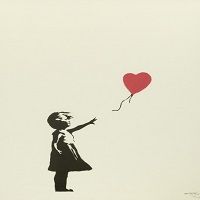
\includegraphics[width=0.75\textwidth]{banksy.jpg}
	}
	\caption[VoltageMatching]{Interconnection of two audio units\,(left) - voltage divider\,(right)\footnotemark}
	\label{fig:VoltageMatching}
\end{figure}
\footnotetext{URL: http://www.sengpielaudio.com/calculator-bridging.htm [cited 23 August 2018]}

\subsubsection{Balanced and Unbalanced transmission}

For the transmission of audio signals, two cable types are commonly used.
Unbalanced cables consist of the centred signal wire and the shield, which is the conductor for the signal return as well.
A shielded cable protects the signal from electromagnetic and radio interference.
This noise rejection is only efficient up to a maximum length of 4,5\,-\,6\,meter, due to the fact that
the wire also acts as an antenna and picks up noise again\footnote{https://ask.audio/articles/music-studio-essentials-understanding-balanced-vs-unbalanced-xlr-cables [cited 25 August 2018]}.
Unbalanced cables are often used to connect an electric guitar or a microphone to an amplifier.
In the domain of consumer audio, they are widely spread.

 
The balanced cable has in contrast to the unbalanced system one additional wire for the signal.
Both wires transmit the same signal with a phase shift of 180 degrees.
In other words, the second wire carries the inverse of the signal.
Along the length of the cable, the two signal wires pick up the same additional noise.
Since the noise parts of the two signals are in phase, both wires can be connected to a differential
amplifier in the receiving device \cite[p.\,490]{Dickreiter:2014}. By calculating the difference of both signals the noise can be eliminated.

Balanced audio systems can carry much longer cable runs compared to an unbalanced cable.
They are used in professional sound systems or in recording studio environment for connections between
amplifiers and mixing consoles.



\subsubsection{Line Level}\label{cap:TheoryLineLevel}

The line standard is distributed in a wide range of applications.
It standardizes the audio transmission in many fields such as
home entertainment, television broadcasting, and professional recording studios.
It describes the nominal level as a ratio for a suitable interconnection between
devices designed for line level.\\
\\
For the consumer audio application (such as CD / DVD Players) the decibel volts (dBV) are used.
The nominal level for consumer audio is specified as -10\,dBV.
In professional audio systems (e.g. mixing tables in television studios) the decibel unloaded (dBu) with
a nominal level of +4\,dBu is standard.

Table \ref{tab:LineLevels} shows the line levels with the corresponding nominal voltages which can be calculated with eq.\,\ref{eq:dBV} and eq.\,\ref{eq:dBu}.

Input and output of the line connections present unequal impedances.
Both designed to ensure a suitable interconnection from a line output to a line input.
The impedance of an input is typically around 10\,k$\Omega$ while the output impedance is usual
around 100\,$\Omega$ to 600\,$\Omega$\footnote{https://en.wikipedia.org/wiki/Line\_level [cited 26 August 2018]}.
Due to the higher input impedance, the signal level is maximised and the current is kept low.

\begin{table}[H]
\begin{center}
\begin{tabular}{|c|c|c|c|c|}
\hline 
\textbf{Application Field} & \textbf{Nominal level} & \textbf{Nominal level, $\mathrm{V}_{\mathrm{RMS}}$}  \\ 
\hline 
\hline 
Consumer audio & -10\,dBV & 0,316 \\ 
\hline 
Professional audio & +4\,dBu & 1,228 \\ 
\hline 
\end{tabular} 
\caption[ui]{Line levels and their approximate nominal voltages}
\end{center}
\label{tab:LineLevels}
\end{table}

\subsubsection{Instrument Level}

Every passive instrument with an output connector for further amplification provides a
different voltage level\,(see table \ref{tab:LineLevels}). Depending on the instrument type, a variety of transducers are used to transform acoustical vibrations an electrical voltage.
This is the reason why there is not one single voltage level valid for all instruments. 

\begin{table}[H]
\begin{center}
\begin{tabular}{|c|c|}
\hline 
\textbf{Type} & \textbf{Output level/ $\mathrm{mV}_{\mathrm{RMS}}$} \\ 
\hline 
\hline
Ribbon microphone & 0,1 \\ 
\hline 
150-Ohm dynamic microphone & 10 \\ 
\hline 
Fender Precision bass pickup & 150 \\ 
\hline 
Humbucker guitar pickup & 200 \\ 
\hline 
Piezo guitar pickup & 0.5 \\ 
\hline 
\end{tabular} 
\caption{Output levels for passive transducers\,\cite{Winer:2012}}
\end{center}
\label{tab:LineLevels}
\end{table}


Though for an electric guitar the range can be limited.
Depending on several parameters like adjustment of the bridge, string cross section and strength of the string-stroke a pickup can produce an output signal between 10\,mV$_{\mathrm{RMS}}$ and 1\,V$_{\mathrm{RMS}}$\footnote{http://www.muzique.com/lab/pick.htm [cited 26 August 2018]}.
The strumming on an open A string of a \textit{Fender Stratocaster} leads to a measured output-voltage about 72\,mV$_{\mathrm{RMS}}$\,(-22\,dBV or -20\,dBu) (see figure \ref{fig:singleCoilVoltage}). Due to the additional harmonics, in this case the oscilloscope calculates the complex waveform as 480,4\,Hz. 
These values can be taken as an assumption for a regular output voltage level of an electric guitar for further calculations.


The output impedance of electric guitars varies caused by the diverse guitar types and tone control settings.
A guitar pickup is a high impedance inductive source commonly in the range of 10\,$\mathrm{k}\Omega$ to 25\,$\mathrm{k}\Omega$\footnote{https://learn.sparkfun.com/tutorials/proto-pedal-assembly-and-theory-guide/theory-of-operations [cited 26 August 2018]}.


\begin{figure}[H]
	\centering 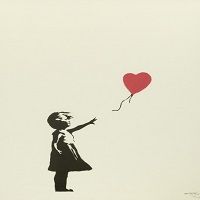
\includegraphics[width=0.5\textwidth]{banksy.jpg}
	\caption[singleCoilVoltage]{Single-coil pickup waveform of an open A 110\,Hz (Fender Stratocaster)\,\cite[p.\,27]{Dailey:2014}}
	\label{fig:singleCoilVoltage}
\end{figure}

\subsubsection{Analog Audio Connectors}

For the interconnection of audio devices, several connectors and cables are used.
In the area of analog audio engineering  connectors such as XLR, RCA, and phone connectors (often
called audio jacks) are to be mentioned. With regard to the following chapters, only the pinout of the relevant audio jacks (see figure \ref{fig:Jacks}) is shown in table \ref{tab:pinoutAudioJacks}.


\begin{figure}[H]
	\centering 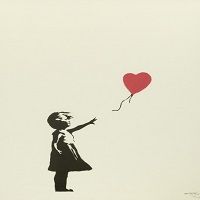
\includegraphics[width=0.25\textwidth]{banksy.jpg}
	\caption[Jacks]{Pinout diagram of a stereo audio jack in TRS standard\footnotemark}
	\label{fig:Jacks}
\end{figure}
\footnotetext{URL: https://robrobinette.com/images/Audio/TRS\_Pinout.jpg [cited 25 August 2018]}

\begin{table}[H]
\begin{center}
\begin{tabular}{|c|c|c|c|}
\hline 
\textbf{ Audio jack} &\textbf{ Pin 1 }& \textbf{Pin 2} & \textbf{ Pin 3} \\ 
\hline 
\hline
6.3\,mm mono & SLEEVE: Ground & TIP: Signal &  - \\ 
\hline 
3.5\,mm stereo & SLEEVE: Ground & TIP: Signal (Left) & RING: Signal (Right) \\ 
\hline 
\end{tabular} 
\caption{Pinout of audio jacks}
\end{center}
\label{tab:pinoutAudioJacks}
\end{table}

\section{Raspberry Pi and Audio-HAT}\label{cap:TheoryPi}

The Raspberry Pi is a single-board computer developed by the Raspberry Pi Foundation.
By March 2017 over 12,5\,million Raspberry Pis were sold, making it one of the best-selling
"general purpose computer" behind Apple Macintosh and Microsoft Windows PCs\footnote{https://www.theverge.com/circuitbreaker/2017/3/17/14962170/raspberry-pi-sales-12-5-million-five-years-beats-commodore-64 [cited 26 August 2018]} .

The first generation "Raspberry Pi 1 Model B" in 2012 came with a processor
speed of 700\,MHz, while the newer processors are running with up to 1,4\,GHz.
For this thesis the widely spread "Raspberry Pi 3 Model B" with a 1,2\,GHz Quad Core Processor is used.
A variety of operating systems like Android Things, Debian or the Debian-based Raspian can be installed 
via the SD-card reader.
Equipped with many onboard interfaces, such as GPIO and display ports, the Pi can be used for a vast number of applications.
\\
A major shortcoming is the analog audio output, which is designed as a 3.5mm audio jack.
It provides a Signal-to-Noise ratio\,(SNR) of 65,5\,dBA\,\cite[pp.\,72-74]{Strom:2015}, which leads to a very weak sound quality.
In addition to that, the Pi is not fitted with an analog audio input.

Therefore Sebastian Albers developed in the context of his bachelor thesis\,\cite{Albers:2017} an Audio-HAT
(Hardware Attached on Top). The HAT extends the Raspberry Pi with professional analog stereo audio in- and output. Also placed on the HAT are the analog-to-digital conversion and the digital-to-analog conversion with a digital word size of 24\,Bit and a maximum sampling frequency of 192\,kHz.The SNR has been improved to 97\,dB\,\cite[p.\,94]{Albers:2017}.
Due to Albers achievements, the Raspberry Pi is therefore capable of digital signal processing.

\begin{figure}[H]
	\centering 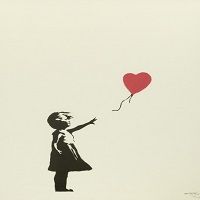
\includegraphics[width=0.65\textwidth]{banksy.jpg}
	\caption[PiandHAT]{Raspberry Pi Model 3B and Audio-HAT \cite[p.\,65]{Albers:2017}}
	\label{fig:PiandHAT}
\end{figure}



\section{Digital Signal Processing}

For the manipulation or processing of analog signals, the digital signal processing is often used. Due to the greatly reduced prices for microelectronics and mass-production of digital circuits, the 
digital signal processing is widely distributed \cite[p.\,101]{Werner:2010}.\\
Figure \ref{fig:DSPScheme} visualizes the process in the context of digital audio effects\,(DAFX) which are part of this thesis. The analog signal $x(t)$ is a continuous-time signal carrying the information as electric pulses of varying amplitude. For the digital signal representation as a discrete-time signal $x(n)$ of the analog signal, an ADC is needed.
The digitization consists of two steps: sampling and quantization.\\
The DAFX box, representing the digital system, performs a manipulation of the sequence of samples $x(n)$ in this case by halving the values. The processed digital signal $y(n)$ is then passed to the DAC for the reconstruction of the analog signal $y(t)$.

\begin{figure}[H]
	\centering 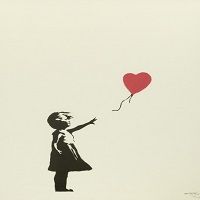
\includegraphics[width=1\textwidth]{banksy.jpg}
	\caption[DSPScheme]{Scheme of digital signal processing \cite[p.\,3]{Zolzer:2002}}
	\label{fig:DSPScheme}
\end{figure}


\subsection{Digital Signals}
\subsubsection{Sampling}
The sampling rate $f_\mathrm{s}$ is the number of samples obtained per second in Hertz.
For the sampling of the analog amplitudes on an equidistant grid along the horizontal time axis, the Nyquist-Shannon sampling theorem (\ref{eq:Nyquist}) must be respected.
It defines that $f_\mathrm{s}$ must be higher than twice the maximum frequency $f_{\mathrm{max}}$ of the analog signal.
If this condition is satisfied, the signal can be reconstructed from its samples.
Not fulfilling the theorem, the sampling could lead to the aliasing effect \cite[p.\,103]{Werner:2010}.

\begin{equation}
f_\mathrm{s} > 2\cdot f_{\mathrm{max}} 
\label{eq:Nyquist}
\end{equation}


\subsubsection{Quantization}

For the amplitudes of the analog signal, discrete values are allocated.
They are represented by numbers $x(n)$ along the vertical axis symbolized by dots\,(see figure \ref{fig:DSPScheme}).
The digital resolution, or the vertical scaling, depends on the defined bit depth.
A higher bit depth leads to a minimized quantization error.
For example, in a 24\,bit representation of sample amplitudes the quantization is in the integer number range between -2$^{24}$ to 2$^{24}$-1.
The maximum digital value is defined as 0 decibels to full scale\,(dbFS). Based on that, the digital amplitude levels can be described in relation to a defined maximum.


\subsubsection{Discrete Fourier transform}

For the conversion of signals from the time-domain to the frequency-domain the 
discrete Fourier function\,(DFT) is used\,(eq. \ref{eq:DFT}). Based on that the calculation of the Fourier
transform of a signal can be done by a computer. The sequence $x(n)$ of $N$ complex numbers is
transformed to the frequency-domain $X(k)$.
In addition to DFT, a more efficient way to perform the transformation is the fast Fourier transform (FFT).
The algorithm is basically just an optimized DFT with a significant reduction of the number of multiplications.
It is a mathematical technique of enormous  technological importance because it allows powerful spectrum analysis on inexpensive microcomputers.\\


\begin{equation}
X(k) =\mathrm{ DFT}[x(n)] = \sum_{n=0}^{N-1} x(n)e^{-j2\pi nk/N}
\label{eq:DFT}
\end{equation}
\begin{center}
$ k=0,1,...,N-1$
\end{center}



\subsection{Digital Systems}

The processing of the digital input signal $x(n)$, provided by the ADC, takes place in the digital system.
An implemented algorithm processes every sample by performing mathematical operations.
The result of the processing is the output signal $y(n)$.


\subsubsection{Impulse Response}

The reaction of a system triggered by a short-time signal is defined as the impulse response\,(see \ref{fig:ImpulseResponse}).
The impulse can be modelled with the Dirac delta function $\delta(n)$ as a test signal.
As a result, the output signal is the impulse response $h(n)$.


\begin{figure}[H]
	\centering 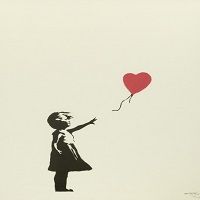
\includegraphics[width=1\textwidth]{banksy.jpg}
	\caption[ImpulseResponse]{Impulse response $h(n)$ as a time domain description \cite[p.\,18]{Zolzer:2002}}
	\label{fig:ImpulseResponse}
\end{figure}


\subsubsection{Transfer Function}

In the time-domain, the behaviour of a digital system can be described with the impulse response.
The reaction of the system in the frequency domain can be described as well.
A system can reject, pass and enhance certain frequencies included in the input signal spectrum \cite[p.\,21]{Zolzer:2002}.
The Transfer function (\ref{eq:TransferFu}) describes the frequency domain behaviour.
It results by applying the Z-transform (\ref{eq:ZTrans}) which is mapping the discrete signal into a complex frequency domain representation. At this point, the complex Z plane is not explained in detail because it is not relevant for this thesis.

%\begin{itemize}
%\color{red}
%\item \textbf{\huge Maybe PCM and iS2}
%\end{itemize}

\begin{equation}
X(z) = \sum_{n=-\infty}^{\infty} x(n)\cdot z^{-n}
\label{eq:ZTrans}
\end{equation}

\begin{equation}
H(z) = \sum_{n=-\infty}^{\infty} h(n)\cdot z^{-n}
\label{eq:TransferFu}
\end{equation}

\section{Guitar Effects}

Guitar players often want to highlight their own performance by applying specific sounds.
The manipulation of the guitar sound via tone controls is very limited.
Therefore to enhance the sound, effect units are widely spread.
The units are connected between the guitar output and the input of an amplifier.
Inside the unit the analog or digital signal processing takes place, changing the signal in the time-domain and/or in the frequency domain. A selection of popular guitar effect is depicted in table\,\ref{tab:guitarEffects}. In this section, the delay and distortion are described in more detail.


\begin{table}[H]
\begin{center}
\begin{tabular}{|c|p{10cm}|}
\hline 
\textbf{Effect}  & \textbf{Description} \\ 
\hline 
\hline
Clean &  No effect applied to the signal. Simple pass through \\ 
\hline 
Equalizer & Variation of the total frequency spectrum. Adjusts specific frequency ranges \\ 
\hline
Delay & Time effect. Multiplication of the signal with a changed delayed copy of itself in the time domain.
 Creating an echoing sound \\ 
\hline 
Chorus & Modulation effect. Comparable with the delay but in addition to that the frequency of each tone is modified \\ 
\hline 
Tremolo & Manipulation of the amplitude. Varies volume of the sound very quickly over time\\ 
\hline 
Boost & Increases the output signal of the guitar. Ideally used during solos \\ 
\hline 
Overdrive & Signal amplitude is limited by using soft clipping. Creating a rounded but cropped wave and
a distorted sound \\ 
\hline
Distortion & Signal amplitude is limited by using hard clipping. Leads to a full and saturated sound \\ 
\hline
Fuzz & Signal amplitude is amplified and cut off at the same time. Almost sounds like an overstrained speaker and leads to the most extreme distorted sound\\ 
\hline
\end{tabular} 
\end{center}
\caption{List of popular guitar effects}
\label{tab:guitarEffects}
\end{table}


\subsection{Delay}

In technology, a delay is often associated to be a negative effect in terms of signal transmission or processing. From an artistic point of view, the delay effect can improve the sound experience.
In a comparable way that a sound benefits from a naturally reverberant space, a delay effect unit can create an echoing sound.
A famous example of the usage in popular music is \textit{Pink Floyd - Run like hell} \footnote{D.Gilmour/R.Waters (PinkFloyd) "Run like Hell".\textit{The Wall}. Harvest Records,1980.LP }.
The basic principle of a delay effect unit is shown in figure \ref{fig:DelaySimple}.

The resulting output signal is the addition of the two signal paths: The \textit{Bypass Curcuit} and the \textit{Delay Line}.
Due to the \textit{Bypass Curcuit} the guitar signal is passed forward to the output without any manipulation. Besides that, the \textit{Delay Line} consists of recordings of the input signal and the recordings back from the \textit{Feedback Line}. As a result, the sound is enhanced with a decaying echo.




\begin{figure}[H]
	\centering 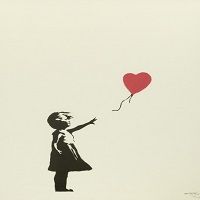
\includegraphics[width=0.5\textwidth]{banksy.jpg}
	\caption[DelaySimple]{Block diagram of the signal-flow for a typical simple delay-line tied to an electric guitar\,\cite[p.\,124]{Hodgson:2010}}
	\label{fig:DelaySimple}
\end{figure}

\subsection{Distortion}

After the invention of the electric guitar, musicians looked for a way to create a louder and heavier sound. On one hand, they boosted the gain level of the guitar by experimenting with new pickups. On the other hand, they increased the volume inside on an amplifier until the vacuum tubes compressed and distorted the guitar signal. As a result, the distorted sound became one of the most important guitar effects and led to the birth of \textit{Rock and Roll}.
For instance, a typical distortion sound is used in the song \textit{In Bloom} by the band \textit{Nirvana}\footnote{K.Cobain (Nirvana) "In Bloom".\textit{Nevermind}. Geffen Records,1991.LP }.

Any deviation of an output signal from the corresponding input signal is called distortion.
There are two kinds of distortion to be distinguished: Linear and nonlinear (see \ref{fig:nonlinearScheme}).

\begin{figure}[H]
	\centering 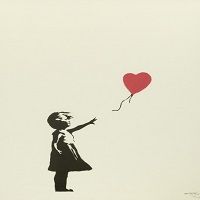
\includegraphics[width=1\textwidth]{banksy.jpg}
	\caption[nonlinearScheme]{Input and output signals of a linear and nonlinear system \cite[p.\,94]{Zolzer:2002}}
	\label{fig:nonlinearScheme}
\end{figure}


\subsubsection{Linear Distortion}
Linear distortion appears when the processing does not affect the original waveform of the signal but a change in amplitude or phase. A simple example is a volume adjustment with no influence on the tone quality. Also, an equalizer for the amplification and/or attenuation of the frequency range is assigned to the linear systems. In addition to that, they occur by using frequency-dependent amplifiers and capacitive or inductive voltage dividers, which do not produce further harmonics \cite{Sengpiel:2007}.

\subsubsection{Nonlinear Distortion}
A nonlinear system affects an output signal that is strongly shaped. In regard to the distortion effect defined in table \ref{tab:guitarEffects} the method of \textit{hard clipping} is to be mentioned here. Nonlinear distortions are caused by curved characteristic lines of semiconductors and vacuum tubes \cite{Sengpiel:2007}. According to that, these systems create harmonic frequency components that are not part of the input signal.\\

Depending on the symmetry of the components's characteristic lines, different parts of the harmonics are amplified.\\
A symmetrical cubic characteristic line highlights the odd integer multiples of the fundamental frequency $f_1$, thus 3$\cdot f_1$,\,5$\cdot f_1$,\,7$\cdot f_1$ and so on.\\
Unsymmetrical quadratic lines lead to even integer multiples such as 2$\cdot f_1$,\,4$\cdot f_1$,\,6$\cdot f_1$.

\subsubsection{Total Harmonic Distortion}

As an indication for the nonlinearity of a system, the total harmonic distortion\,(THD) is defined.
It specifies the relative amount of harmonics expressed in percentage\,(\ref{eq:THD}) or decibel\,(\ref{eq:THDdb}) and describes the extent of distortion\,\cite{Rohde:2005}.
If the amplitude of the fundamental is $U_1$, and the amplitude of the $n$-th harmonic is $U_i$, then the 
THD for $n$ harmonics can be defined.
A lower THD means a more accurate reproduction of the input signal.\\


\begin{equation}
\mathrm{THD}_{\mathrm{dB}} = 20 \cdot \mathrm{log} \frac{\sqrt{\sum\limits_{i=2}^{n} \cdot {U_i}^2}}{{\sqrt{\sum\limits_{i=1}^{n} \cdot {U_i}^2}}}
\label{eq:THDdb}
\end{equation}

\begin{equation}
\mathrm{THD}_{\%} = 10^{\frac{\mathrm{THD/dB}}{20}} \cdot 100
\label{eq:THD}
\end{equation}

Besides the THD, a much more common method for the evaluation of an audio device performance is the total harmonic distortion plus noise\,(THD+N) measurement. In contrast to the THD, the harmonics are measured - by taking into account the resulting noise (see equation \ref{eq:THDdbplusN}).
As well as the THD measurement the THD+N is expressed as an RMS level.

\begin{equation}
\mathrm{THD}_{\mathrm{dB}} = 20 \cdot \mathrm{log} \frac{\sqrt{\sum\limits_{i=2}^{n} \cdot {U_i}^2 + {U_{noise}}^2}}{{\sqrt{\sum\limits_{i=1}^{n} \cdot {U_i}^2}}}
\label{eq:THDdbplusN}
\end{equation}


